% Appendix E -- Answers to Exercises
\chapter{Answers to Exercises}

\section{From Chapter 1}
\begin{enumerate}
	\item Compare and contrast population statistics versus sample statistics.
	

	{\small \texttt{Population statistics involve data from the entire universe of a subject under study, and are denoted by Greek letters.  Sample statistics, on the other hand, involve a relatively small number of randomly selected samples from a pop\-u\-la\-tion. They are denoted by English letters and only infer characteristics of the population they represent.}}

	
	\item What does the term \textit{inferential statistics} mean?
	
	
	{\small \texttt{Inferential statistics are those that infer, or deduce from sample evidence. They are estimates of the true nature, or value of a population char\-ac\-ter\-is\-tic.}}

	
	\item What is the difference between location statistics and variation statistics?
	

	{\small \texttt{Location statistics describe the magnitude of a dimension, for example, as if on a number line. This would also relate to a two-dimensional parameter, such as x-y coordinates, with a desire to be ``on target'' as if in the center of a bulls-eye. Variation statistics describe how precise a measure has been, where closely associated locations have low variance and widely spread data have high variance, or error.}}

	
	\item How are location statistics and variation statistics related to accuracy and precision?  
	
	
	{\small \texttt{Accuracy denotes close proximity of an average value of multiple observations to a target value, or a location of desire.  Precision denotes re\-pea\-ta\-bil\-i\-ty and re\-pro\-duc\-i\-bil\-i\-ty such that each time a measurement is taken very similar location results are observed in close proximity as a group as opposed to being widely scattered.} }
	
\end{enumerate}


\section{From Chapter 2}
\begin{enumerate}
	\item Describe a work environment from your past experiences in which data were collected, some analysis done, and results reported.  Specify how the data were reported, number of samples evaluated, calculations performed, etc.
	

	{\small \texttt{An example in a typical laboratory environment might be taking measurements of mass on an analytical lab balance. Typically multiple samples are tested, perhaps three to five samples. Typically the analyst reports an average (mean) value of the individual observations by summing the numerical results and dividing by the number of samples.}}

	\item What is a \textit{confidence interval}?
	

	{\small \texttt{A confidence interval is a range of values that encompasses a mean value of measurements. The range reported relates to a specific level of confidence, e.g. 95\% confidence. Different confidence levels correspond to different ranges.  For example the range of a 99\% confidence interval is wider than the 95\% interval for the same data.}}

	
	\item How does one find the correct value for $ t $ in a table of the Student's t distribution (see Appendix \ref{AppendixA})?
	

	{\small \texttt{To find the appropriate table value, the analyst must first have determined the degrees of freedom available based on sample size. For example if evaluating a set of five observations, the degrees of freedom would be N-1, or 4 degrees of freedom. The second parameter needed is the desired confidence level. Often this is 95\%, but any level of confidence may be chosen.  Once these two parameters are known, the table is used to obtain the Student's t statistic.}}

	
	\item When reporting a result with 95\% confidence, what is the chance that this statement is wrong?
	

	{\small \texttt{The probability that a result reported with 95\% confidence is wrong, is simply 100\% - 95\% = 5\% chance of being wrong. While this is entirely possible, it is unlikely at such a low value.}}

\end{enumerate}

\section{From Chapter 3}
\begin{enumerate}
	\item Are these samples the same or are they different?
	
	\begin{tabular}{|c|c|}
		\hline \textbf{Sample 1} & \textbf{Sample 2} \\ 
		\hline 14.59 & 14.62 \\ 
		\hline 15.01 & 14.69 \\ 
		\hline 15.47 & 14.95 \\ 
		\hline 15.56 & 14.76 \\ 
		\hline 15.05 & 14.87 \\ 
		\hline 
		
	\end{tabular}\\
\newpage
\textbf{R code:}

\begin{lstlisting}
# create function to perform the t-test

t.test.fromRawData <- function(mu,n,s){-diff(mu) / sqrt( sum( s^2/n ) )}

# Load a Comma Separated Value (CSV) file saved from a spreadsheet for data input to a data frame

data <- read.csv("TwoMeans.csv", header = TRUE)

# Calculate the mean and standard deviation for each sample

x1 <- mean(data[["Sample.1"]])
x2 <- mean(data[["Sample.2"]])
s1 <- sd(data[["Sample.1"]])
s2 <- sd(data[["Sample.2"]])

# create vectors from above variables to load into the function

mu <- c(x1,x2)
s <- c(s1,s2)

# define total number of observations

n <- nrow(data["Sample.1"]) + nrow(data["Sample.2"])

# define the level of confidence desired (nominally 95%)

ConfLevel <- 0.95

# Use the fuction to compute the result of the t-test

result <- t.test.fromRawData(mu,n,s)

tablevalue <- abs(qt((1-ConfLevel)/2, n))

cat("Student's t-test to compare two sample means", "\n \n")
	
cat("Raw data:","\n")

cat("Sample 1:", data[["Sample.1"]]," Mean: ", x1, " Std. Dev: ", s1, "\n\n")

cat("Sample 2:", data[["Sample.2"]]," Mean: ", x2, " Std. Dev: ", s2, "\n\n")

cat("The Student's t value is:", result,"\n\n")

if (result > tablevalue)  

	cat(" which is greater than the critical value,", tablevalue, "thus we must reject the null hypothesis as this is evidence that the two samples are significantly different, at the", ConfLevel*100, "% confidence level.") 
else 

	cat(" which is less than the critical value,", tablevalue, "so we must accept the null hypothesis as we have no evidence that the samples are different at the", ConfLevel*100, "% confidence level.")
\end{lstlisting}


\textbf{Output:}


{\small \texttt{Student's t-test to compare two sample means} 

\texttt{Raw data: }\\
\texttt{Sample 1: 14.59 15.01 15.47 15.56 15.05}\\
\texttt{Mean:  15.136   Std. Dev:  0.3913822}

\texttt{Sample 2: 14.62 14.69 14.95 14.76 14.87}\\
\texttt{Mean:  14.778   Std. Dev:    0.1333042}

\texttt{The Student's t value is: 2.738095}

\texttt{which is greater than the critical value, 2.228139 thus 
we must reject the null hypothesis as this is evidence 
that the two samples are significantly  different, at 
the 95\% confidence level.}}

\newpage
	\index{confidence}
	\item Calculate $ \bar{x}, s, $ and 95\% confidence intervals for \textbf{Sample 1} and \textbf{Sample 2} from the table above.

\textbf{R code:}	
\begin{lstlisting}
# Load a Comma Separated Value (CSV) file saved from a spreadsheet for data input to a data frame

data <- read.csv("TwoMeans.csv", header = TRUE)

# Calculate the mean and standard deviation 
x1 <- mean(data[["Sample.1"]])
x2 <- mean(data[["Sample.2"]])
s1 <- sd(data[["Sample.1"]])
s2 <- sd(data[["Sample.2"]])

# create vectors from above variables to load into the function
mu <- c(x1,x2)
s <- c(s1,s2)
n <- nrow(data)

# Calculate the interval
error <- qt(0.975,df=n-1)*s/sqrt(n)
left <- mu-error
right <- mu+error

# Produce the output
cat("Mean, Standard Deviation, and 	Confidence Intervals:","\n \n")

cat("Sample 1:", "Mean: ", x1, "  Std. Dev: ", s1, "\n")
cat("Confidence interval:", left[1], "to", right[1], "\n \n")

cat("Sample 2:", "Mean: ", x2, "  Std. Dev: ", s2, "\n")
cat("Confidence interval:", left[2], "to", right[2])
\end{lstlisting} 

\textbf{Output:}

{\small \texttt{Mean, Standard Deviation, and Confidence Intervals:} 

\texttt{Sample 1: Mean:  15.136   Std. Dev:  0.3913822} 
\texttt{Confidence interval: 14.65003 to 15.62197}

\texttt{Sample 2: Mean:  14.778   Std. Dev:  0.1333042 }
\texttt{Confidence interval: 14.61248 to 14.94352}}



	\item Plot the mean values using a line chart (\textbf{Sample 1}, \textbf{Sample 2}, and \textbf{Sample 3} from the table below) with 95\% confidence intervals as error bars.\index{mean}
	
	\begin{tabular}{|r|r|r|r|}
		\hline Obs. & \textbf{Sample 1} & \textbf{Sample 2} & \textbf{Sample 3} \\ 
		\hline 1 & 7.5 & 7.2 & 7.7 \\ 
		\hline 2 & 7.9 & 7.4 & 7.9 \\ 
		\hline 3 & 8.3 & 6.9 & 8.3 \\ 
		\hline 
	\end{tabular} 

\bigskip
\textbf{R code:}
\begin{lstlisting}
# plotmeans requires package "gplots"

library(gplots)

# Load a Comma Separated Value (CSV) file saved from a spreadsheet for data input to a data frame

data <- read.csv("ThreeSamples.csv", header = TRUE)

obs <- data.matrix(data)

Sample <- 1:3

plotmeans(t(obs)~Sample, 
xlab ="Sample #", 
ylab ="Mean value",
n.label = FALSE,
main="Chapter 3, exercise #3 plot")
\end{lstlisting}

The output of the code above is given in figure \ref{Ex3}.

\begin{figure}
	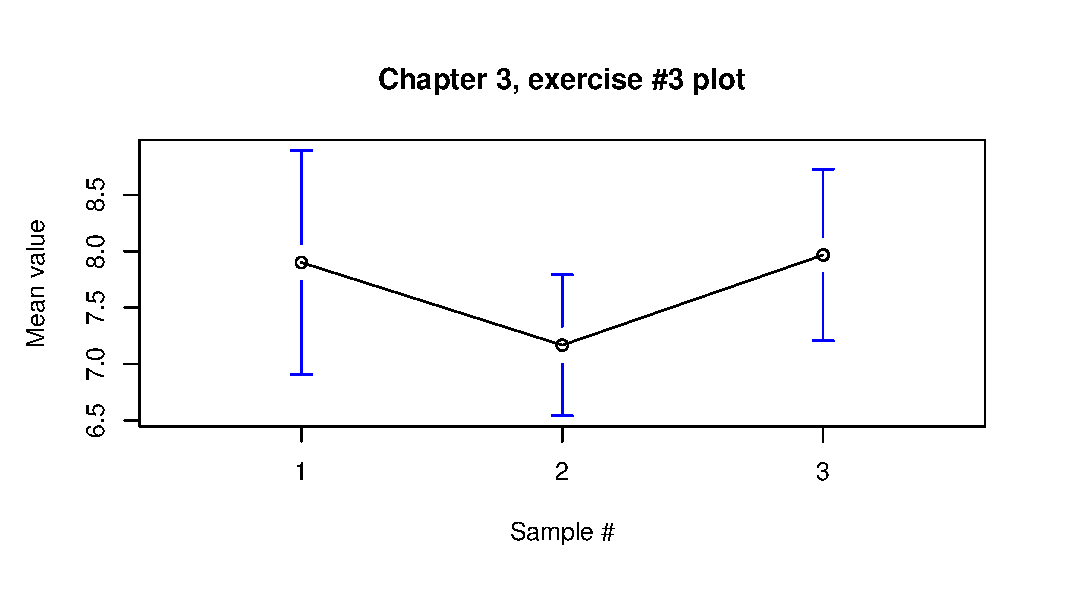
\includegraphics[height=3in, width=\linewidth]{Ex3plot.eps}
	\caption{Plot of mean values with 95\% confidence interval error bars.}\label{Ex3}
\end{figure}
	
\end{enumerate} 